% D.36 △ABC：∠B=45°，∠C=30°，BC=10+10√3；AD⊥BC 于 D
\documentclass[tikz,border=4pt]{standalone}
\usepackage{ctex}
\usepackage{amsmath}
\usetikzlibrary{calc}
\begin{document}
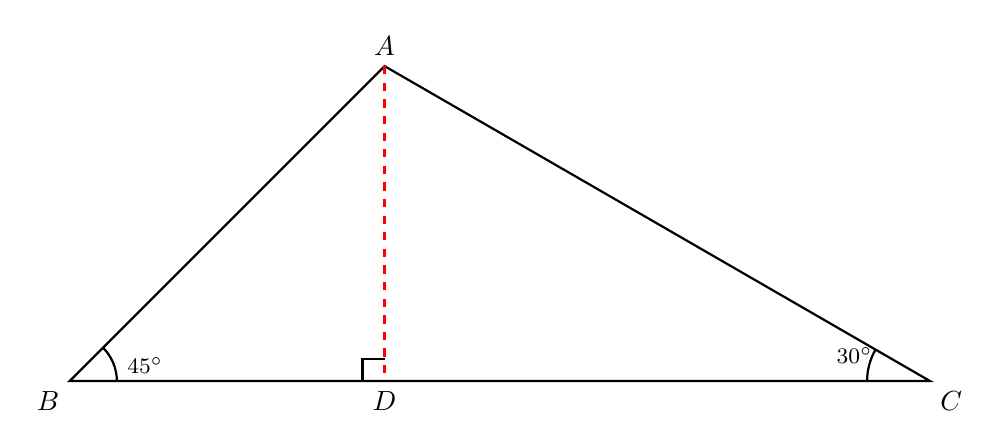
\begin{tikzpicture}[scale=0.4, thick]
  % 设 AD=h。BD = h/tan45° = h；DC = h/tan30° = h√3；BD+DC = h+h√3 = 10+10√3 → h=10
  \pgfmathsetmacro{\h}{10}
  \coordinate (B) at (0, 0);
  \coordinate (D) at (\h, 0);
  \coordinate (C) at ({\h + \h*sqrt(3)}, 0);
  \coordinate (A) at (\h, \h);

  \draw (A) -- (B) -- (C) -- cycle;
  \draw[red, dashed] (A) -- (D);
  \draw (\h-0.7, 0) -- (\h-0.7, 0.7) -- (\h, 0.7);

  \draw (1.5, 0) arc[start angle=0, end angle=45, radius=1.5];
  \node at (2.4, 0.5) {\footnotesize $45^\circ$};
  \draw ({\h + \h*sqrt(3) - 2}, 0) arc[start angle=180, end angle=150, radius=2];
  \node at ({\h + \h*sqrt(3) - 2.4}, 0.8) {\footnotesize $30^\circ$};

  \node[above]       at (A) {$A$};
  \node[below left]  at (B) {$B$};
  \node[below right] at (C) {$C$};
  \node[below]       at (D) {$D$};
\end{tikzpicture}
\end{document}
